\documentclass[manual/man.tex]{subfiles}
\section{Fjärrstyrning}
För att styra bilen måste man först initiera en trådlös länk mellan bilens
kommunikationsmodul och datorn man använder. Detta görs genom att starta en
server via kommandot make comm.remote. När servern är på kan man ansluta till
bilen via det grafiska användargränssnittet.
    
\subsection{Grafiskt Användargränssnitt}
Det finns ett grafiskt användargränssnitt som man kan använda för att koppla
upp sig till bilen. För att starta gränssnittet kör man filen main.py.

\subsubsection{Anslutning}
För att ansluta till den startade servern navigerar man till
System-Server-Connect. 

\begin{figure}[h]
    \centering
    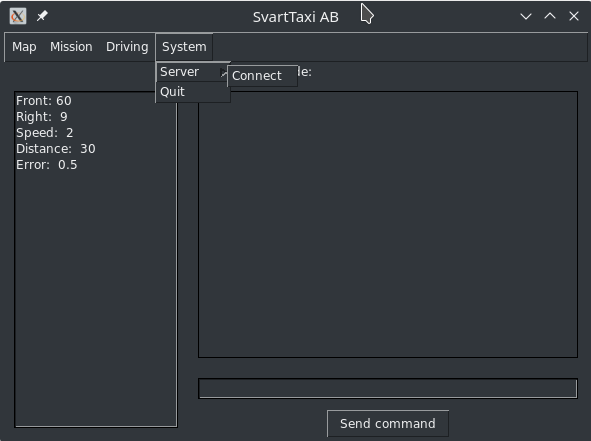
\includegraphics[width=0.6\linewidth]{manual/figures/system_menu.png}
    \caption{Hur man navigerar för att ansluta till servern.}
    \label{fig:sys_menu}
\end{figure}

\noindent
Efter att man tryckt på Connect kommer en ruta upp där
man kan skriva in en IP-adress.

\begin{figure}[h]
    \centering
    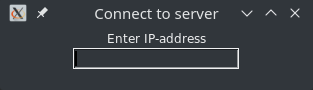
\includegraphics[width=0.6\linewidth]{manual/figures/enter_ip.png}
    \caption{Rutan som kommer upp när man trycker på \textit{Connect}.}
    \label{fig:connect}
\end{figure}

\noindent
IP-adressen som ska skrivas in är samma IP-adress bilen är uppkopplad till. För
att bekräfta sitt val av IP måste enter-knappen på tangentbordet tryckas ner.
Ett meddelande skrivs ut i terminalen efter att man trycker på enter, med ett
felmeddelande ifall klienten inte lyckas anslutas till bilen

\subsubsection{Körning}
Efter att ha anslutit till bilen kan man välja ifall man vill styra bilen
manuellt eller ifall man vill att bilen skall köra autonomn. För att välja
detta navigerar man till Driving-Manual respektive Driving-Auto.

\begin{figure}[h]
    \centering
    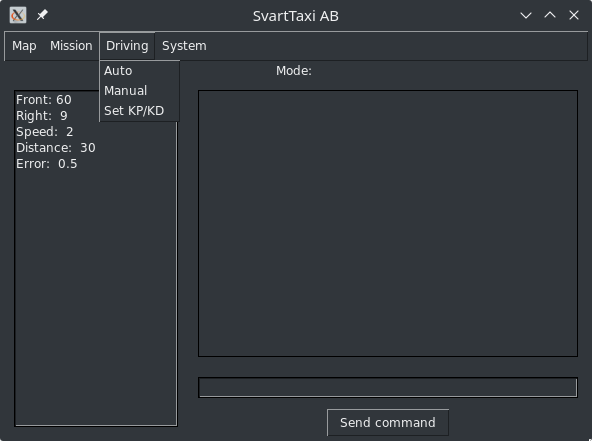
\includegraphics[width=0.6\linewidth]{manual/figures/driving_menu.png}
    \caption{Hur man navigerar för att byta körläge.}
    \label{fig:driving_mode}
\end{figure}

\noindent
För att ändra reglerparametrarna navigerar man till Driving-Set KP/KD. En ny
ruta kommer upp där man kan ange värden för parametrarna man vill ändra. För
att bekräfta sitt val av KP/KD måste man, precis som tidigare, trycka ner
enter-knappen på tangentbordet.

\subsubsection{Banan}
Banan representeras av noder och enkelriktade kanter, där varje nod
representerar en stopp-, rondell- eller parkeringslinje på banan. Varje kant
representerar en vägfil på banan. För att skapa noder högerklickar man i den
stora rutan på gränssnittet och navigerar till Create. Där finns flera olika
valalternativ. Man kan välja antingen Stopline, Parking eller Roundabout, där
Stopline är representerade av röda cirklar, Parking av gula cirklar och
Roundabout av blå cirklar på användarsnittet. Se Figur \ref{fig:create_node}.

\begin{figure}[H]
    \centering
    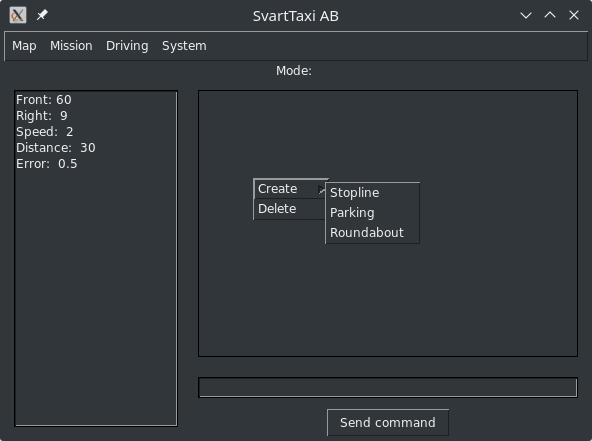
\includegraphics[width=0.6\linewidth]{manual/figures/create_node_menu.png}
    \caption{Hur man navigerar för att skapa olika noder.}
    \label{fig:create_node}
\end{figure}


För att skapa kanter måste man först ha skapat 2 noder. Om man vänsterklickar
på en nod blir den grön, detta betyder att noden är markerad. Om man
vänsterklickar på en annan nod medan en nod är markerad kommer en ny ruta upp
där man kan mata in kostnaden på kanten. Kostnaden representerar längden på
vägfilen i banan. 

\begin{figure}[h]
    \centering
    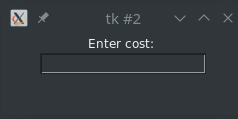
\includegraphics[width=0.6\linewidth]{manual/figures/enter_cost.png}
    \caption{Rutan som kommer fram när man ska skapa en kant.}
    \label{fig:create_edge}
\end{figure}

Rondeller på banan representeras en nod för varje infart och en nod för varje
utfart. En rondell med 3 infarter/utfarter representeras med 6 noder, en
rondell med 4 infarter/utfarter representeras med 8 noder, och så vidare. Alla
kanter inom rondellen är endast riktade åt ett håll. en rondell kan se ut som
visat i Figur \ref{fig:create_edge}.
